\documentclass[10pt,a4paper]{exam}
\usepackage[utf8]{inputenc}
\usepackage{amsmath}
\usepackage{commath}
\usepackage{amsfonts}
\usepackage{amssymb}
\usepackage{booktabs}
\usepackage{graphicx}
\usepackage[left=.75in,right=.75in,top=.75in,bottom=.75in]{geometry}

\usepackage{tikz}
\usetikzlibrary{chains}



\author{Ryan Honea}
\title{Time Series Analysis Homework 1}
\printanswers
\begin{document}
\maketitle

\begin{questions}
\question Let $X$ and $Y$ be two random variables with joint pdf $f(x,y) = 3x$ for $0 \leq y \leq x \leq 1$, and zero elsewhere.

\begin{parts}
\part Compute $P(0 < X < 0.5 \cap Y \geq 0.25)$

\begin{solution}
\begin{align*}
P(0 < X < 0.5 \cap Y \geq 0.25) &= \int_{0.25}^{0.5} \int_{0.25}^x 3x \dif y\dif x\\
		&= \int_{0.25}^{0.5} 3xy \Bigm|_{0.25}^x \dif x\\
		&= \int_{0.25}^{0.5} 3x^2 - \frac{3}{4}x \dif x\\
		&= x^3 - \frac{3}{8}x^2 \Bigm|^{0.50}_{0.25}\\
		&= \left(0.5^3 - \frac{3}{8}0.5^2\right) - \left(0.25^3 - \frac{3}{8}0.25^2\right)\\
		&= \frac{5}{128}
\end{align*}
\end{solution}
\part Compute marginal densities of $X$ and $Y$
\begin{solution}
\begin{align*}
f(x) 	&= \int_0^x 3x \dif y				& f(y) 	&=\int_y^1 3x \dif x\\
		&= 3xy \Bigm|_0^x				& 			&= \frac{3}{2}x^2\Bigm|_y^1\\
		&= 3x^2								&			&= \frac{3}{2}(1 - y^2)
\end{align*}
\end{solution}
\end{parts}

\pagebreak

\question Suppose $X$ and $Y$ are random variables with joint probability density function of the form $f(x,y) = x + y$, for $0 \leq x \leq 1$; and $0 \leq y \leq 1$ and zero elsewhere.

\begin{parts}
\part Find the marginal distribution of $X$ and $Y$.

\begin{solution}
\begin{align*}
f(x)	&= \int_0^1 x + y \dif y							& f(y)	&= \int_0^1 x + y \dif x \\
		&= xy + \frac{y^2}{2} \Bigm|_0^1			&			&= \frac{x^2}{2} + xy \Bigm|_0^1\\
		&= x + \frac{1}{2}									&			&= y + \frac{1}{2}
\end{align*}
\end{solution}

\part Compute $E(X)$, $E(Y)$, $Var(X)$, and $Var(Y)$.

\begin{solution}
\begin{align*}
E[X] 	&= \int_0^1 x\left(x + \frac{1}{2}\right) \dif x									& E[Y] 	&= \int_0^1 y\left(y + \frac{1}{2}\right) \dif y\\
		&= \frac{x^3}{3} + \frac{x^2}{4}\Bigm|^1_0						&			&= \frac{y^3}{3} + \frac{y^2}{4} \Bigm|_0^1\\
		&= \frac{7}{12}																&			&= \frac{7}{12}\\
Var[X] 	&= E[X^2] - E[X]^2																&	Var[Y]	&= E[Y^2] - E[Y]^2\\
			&= \int_0^1 x^2\left(x + \frac{1}{2}\right) \dif x - \left(\frac{7}{12}\right)^2  & &= \int_0^1 y^2\left(y + \frac{1}{2}\right) \dif y - \left(\frac{7}{12}\right)^2\\
			&= \frac{x^4}{4} + \frac{x^3}{6}\Bigm|^1_0 - \frac{49}{144}	&				&= \frac{y^4}{4} + \frac{y^3}{6}\Bigm|^1_0 - \frac{49}{144}\\
			&= \frac{11}{144}														& &= \frac{11}{144}
\end{align*}
\end{solution}

\part Compute $Cov(X, Y)$.

\begin{solution}
\begin{align*}
Cov(X,Y)	&= E[(X - E[X])(Y - E[Y])] \\
				&= E\left[XY - \frac{7}{12}X - \frac{7}{12}Y + \frac{49}{144}\right]\\
				&= E[XY] - \frac{7}{12}(E[X] + E[Y]) + \frac{49}{144}\\
				&=\int_0^1\int_0^1 x^2y + xy^2 \dif x \dif y - \frac{49}{144}\\
				&= \int_0^1 \frac{y}{3} + \frac{y^2}{2} \dif y - \frac{49}{144} = \frac{2}{6} - \frac{49}{144}\\
				&= -\frac{1}{144}
\end{align*}
\end{solution}

\part Compute $E[(2X - Y)^2]$
\begin{solution}
\begin{align*}
E[(2X - Y)^2] 	&= 4E[X^2] - 4E[XY] + E[Y^2]\\
						&= 4\left(\frac{10}{24}\right) - 4\left(\frac{2}{6}\right) + \frac{10}{24}
						&= \frac{3}{4}
\end{align*}
\end{solution}
\end{parts} \pagebreak

\question Suppose $X$ and $Y$ are random variables with joint probability density function of the form $$f(x,y) = KXe^{-(x+y)/2}, \quad x \geq 0, \quad y \geq 0$$ and zero elsewhere.

\begin{parts}
\part Find the value of $K$.
\begin{solution}
\begin{align*}
1		&= \int_0^\infty \int_0^\infty KXe^{-(x+y)/2}\dif y \dif x\\
		&= \int_0^\infty \left[-2Kxe^{-(x+y)/2}\Bigm|^\infty_0 \right] \dif x &= 2K\int_0^\infty xe^{-x/2} \dif x\\
		&= 2K \left[ \left(-2xe^{-x/2} + 2 \int e^{-x/2}\right) \Bigm|_0^\infty\right] &= 2K \left[ \left(-2xe^{-x/2}  - 4e^{-x/2} \right)\Bigm|_0^\infty\right]\\
1		&= 8K\\
K		&= .125
\end{align*}
\end{solution}
\part Compute $Cov(X,Y)$.
\begin{solution}
Note that $Cov(X, Y) = E[XY] - E[X]E[Y]$, so first we find $E[XY]$.

\begin{align*}
E[XY] 	&= \frac{1}{8} \int_0^\infty \int_0^\infty x^2ye^{-(x+y)/2} \dif y \dif x\\
			&= \frac{1}{8} \int_0^\infty x^2e^{-x/2} \left[ \int_0^\infty ye^{-y/2} \dif y \right] \dif x\\
			&= \frac{1}{8} \int_0^\infty x^2 e^{-x/2} \left[-2ye^{-y/2} - 4e^{-y/2}\right]^\infty_0 \dif x\\
			&= \frac{1}{2} \int_0^\infty x^2 e^{-x/2} \dif x\\
			&= \frac{1}{2} \left[ -2x^2e^{-x/2} + 4 \left( -2xe^{-x/2} - 4e^{-x/2} \right) \right]^\infty_0\\
			&= 8\\
\end{align*}

Now, we need the marginal distributions for each of them to find $E[X]$ and $E[Y]$.
\begin{align*}
f_x(x) 	&= \frac{1}{8}xe^{-x/2}\int_0^\infty e^{-y/2} \dif y			& f_y(y) 	&= \frac{1}{8}e^{-y/2}\int_0^\infty xe^{-x/2} \dif x\\
			&= \frac{1}{4}xe^{-x/2}													&			 	&= \frac{1}{2}e^{-y/2}\\
E[X]		&= \frac{1}{4} \int_0^\infty x^2e^{-x/2} \dif x					& E[Y]		&= \frac{1}{2}\int_0^\infty ye^{-y/2}\\
			&= 4																				&				&= 2
\end{align*}

Based on these results, the covariance is
\begin{align*}
Cov(X,Y) 	&= E[XY] - E[X]E[Y]\\
				&= 8 - 4*2\\
				&= 0
\end{align*}


\end{solution}
\pagebreak

\part Find $E[XY^2$].
\begin{solution}
\begin{align*}
E[XY^2]	&= \frac{1}{8} \int_0^\infty x^2y^2 e^{-(x+y)/2} \dif y \dif x\\
				&= \frac{1}{8} \int_0^\infty x^2e^{-x/2} \left[\int_0^\infty y^2e^{-y/2} \dif y \right] \dif x\\
\end{align*}

Note that the elements within the bracket are similar to the second moment of the exponential distribution,  that is, we can write that as 2 times the variance plus the mean squared for $\lambda = 0.5$. For $Exp(\lambda = 1/2)$, the variance is 4 and the mean is 2, so the values within the brackets result in 16.

\begin{align*}
E[XY^2]	&= \frac{1}{8} \int_0^\infty x^2e^{-x/2} \left[16\right] \dif x\\
				&= 2 \int_0^\infty x^2e^{-x/2} \dif x\\
\end{align*}

The same argument can be made for the above integral and so

$$E[XY^2] = 32$$
\end{solution}
\end{parts}

\pagebreak

\question Consider a random process $X_t = \sin(\frac{2\pi}{100}t + \phi)$.
\begin{parts}
\part Consider $\phi \sim \text{Uniform}(-\pi, \pi)$. Plot the process for $t \in (0,1000)$
\begin{center}
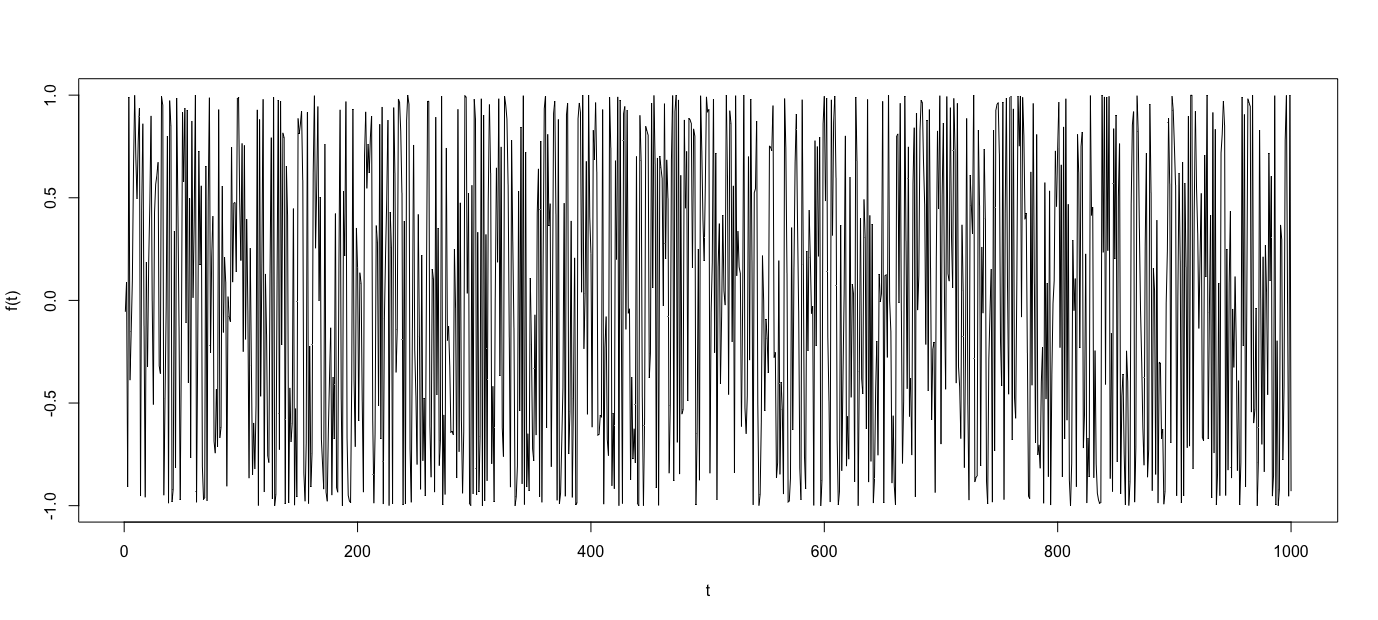
\includegraphics[width=\linewidth]{4a}
\end{center}
\part Consider $\phi \sim \text{Uniform}(0, \pi)$. Plot the process for $t \in (0, 1000)$.
\begin{center}
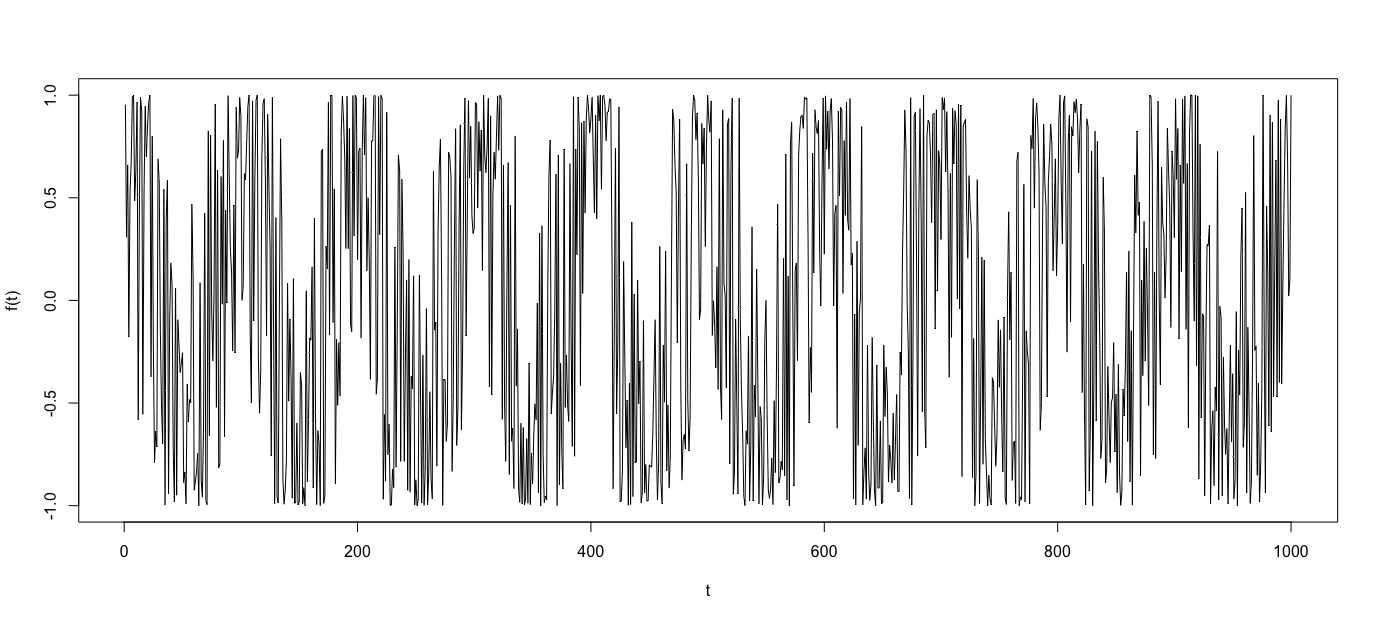
\includegraphics[width=\linewidth]{4b}
\end{center}
\part In terms of mean, what difference do you see in these plots? Explain the difference.

\begin{solution}
The difference in the plot, though slightly in the population mean, is primarily in the means at different neighborhoods. Over time, the mean of (a) appears to be stationary while (b)'s mean seems to fluctuate. This can be shown mathematically. Note first that $E[X_t]$ in (a) is equal to 0 because it is an odd function. For (b), however, this result is different.

\begin{align*}
E[X_t]	&= E\left[\sin\left(\frac{2\pi}{100}t + \phi\right)\right]\\
			&= \int_{0}^\pi  \sin\left(\frac{2\pi}{100}t + \phi\right) \frac{1}{\pi} \dif \phi = \frac{1}{\pi} \int_{0}^\pi  \sin\left(\frac{2\pi}{100}t + \phi\right) \dif \phi\\
			&= \frac{1}{\pi}\left[ -\cos\left(\frac{2\pi}{100}t + \phi\right) \Bigm|^\pi_{0}\right]\\
			&= \frac{1}{\pi}\left[-\cos\left(\frac{2\pi}{100}t + \pi\right) + \cos\left(\frac{2\pi}{100}t + 0\right)\right] = \frac{2}{\pi}\cos\left(\frac{2\pi}{100}t\right)
\end{align*}

So clearly, the expected values of (a) and (b) are different which results in the plots observed.
\end{solution}
\end{parts}
\end{questions}
\end{document}